\chapter{Lecture 24 - The Wave Equation}
\label{ch:lec24}
\section{Objectives}
\begin{itemize}
\item Use separation of variables method to solve the Wave Equation.
\item Illustrate the example solution with MATLAB.
\end{itemize}
\setcounter{lstannotation}{0} %hack to try and re-set annotation counter.

\section{Analytic Solution}
Consider the following boundary value problem based on the wave equation:
\marginnote[1.0cm]{This boundary value problem models a flexible string fixed on both ends with a specified initial displacement, $f(x)$, and initial velocity, $g(x)$.}
\begin{table}
\begin{tabular}{l l}
$\substack{\text{Governing} \\\text{Equation}}: $& $\frac{\partial^2 u}{\partial t^2} = \alpha^2 \frac{\partial^2 u}{\partial x^2}, \ \ \alpha > 0, \ a<x<b$  \\
& \\
$\substack{\text{Boundary} \\ \text{Conditions}}: $& $u(0,t)=0, \ \ u(L,t) = 0, \ \ t>0$\\
& \\
$\substack{\text{Initial} \\ \text{Conditions}}: $ & $u(x,0) = f(x), \ \ u_{t}(x,0) = g(x), \ \ 0<x<L $ \\
\end{tabular}
\end{table}

\vspace{0.25cm}

\noindent We will follow the steps to find the solution using separation of variables.

\vspace{0.5cm}

\noindent\textbf{Step \#1:} Assume a product solution:
\begin{equation*}
u(x,t) = F(x)G(t)
\end{equation*}

\vspace{0.5cm}

\noindent\textbf{Step \#2:} Insert proposed solution into the governing equation:
\begin{align*}
\frac{\partial^2}{\partial t^2}\left[F(x) G(t)\right] &= \alpha^2 \frac{\partial^2 }{\partial x^2}\left[F(x)G(t) \right] \\
FG_{tt} &= \alpha^2 F_{xx}G
\end{align*}

\vspace{4.0cm}

\noindent\textbf{Step \#3:} Separate variables: \marginnote{We assume that $F(x)$ and $G(t)$ are not identically zero throughout the domain, thus dividing by $F(x)G(t)$ is mathematically acceptable.}
\begin{align*}
\frac{FG_{tt}}{\alpha^2 FG} &= \frac{\alpha^2 F_{xx}G}{\alpha^2 FG} \\
\frac{G_{tt}}{\alpha^2 G} &= \frac{F_{xx}}{F} = -\lambda \\
G_{tt} + \alpha^2 \lambda G = 0, \ \ & \ \ F_{xx}+\lambda F = 0
\end{align*}
\marginnote[-2.0cm]{On the middle line we see that $\frac{G_{tt}}{\alpha^2 G}$ is only a function of $y$; $\frac{F_{xx}}{F}$ is only a function of $x$ and yet they must be equal to each other for all values of $x$ and $y$.  The only way this makes sense is if they are both, in fact, constant.  We will denote this constant $-\lambda$.}

\vspace{0.5cm}



\noindent\textbf{Step \#4:} Apply boundary conditions to determine non-trivial product solution(s).  

\noindent The boundary conditions must be applied to the separated equation for $F(x)$.\sidenote{As with the heat equation in Lecture 23, the only way $G(t)$ can satisfy the homogeneous spatial boundary conditions would be for us to set $G(t)=0$.  Thus the product solution would be $u(x,t)=F(x)G(t) = F(x)(0)=0$.  Obviously a trivial solution $u(x,t)=0$ is not what we are looking for.}

\begin{equation*}
F_{xx} + \lambda F = 0, \ \ F(0) = 0, \ \ F(L) = 0, \ \ 0<x<L
\end{equation*}

\noindent We need to examine all possible values of $\lambda$.

\vspace{0.25cm}

\noindent\underline{$\lambda = 0$}:
\marginnote[0.75cm]{This analysis is identical to what we carried out in the last lecture for the heat equation.  It is worth doing this a few times just to make sure you know what you are doing.  After that, you may decide that it is okay to skip to the answer.  It can be risky to ``skip to the answer'' so do not let me tempt you away from the straight-and-narrow path of always thoroughly looking for valid eigenvalues.}
\begin{align*}
F_{xx} &= 0 \\
F(x) &= c_1x + c_2 \\
F(0) &= c_1(0) + c_2 = 0 \\
\Rightarrow & c_2 = 0 \\
F(L) &= c_1(L) = 0 \\
\Rightarrow & c_1 = 0
\end{align*}
Thus we will disregard $\lambda = 0$ since, in that case, only the trivial solution satisfies the governing equation and boundary conditions.

\vspace{0.25cm}

\noindent\underline{$\lambda < 0$}:  Here we will set $\lambda = -\nu^2, \ \ \nu>0$. \marginnote[1.5cm]{Note again that we use the $\cosh()$ and $\sinh()$ form of the solution since the domain is bounded.}
\begin{align*}
&F_{xx} - \nu^2 F = 0 \\
&F(x) = c_1 \cosh{\nu x} + c_2 \sinh{\nu x} \\
&F(0) = c_1 \cancelto{1}{\cosh{0}} + c_2 \cancelto{0}\sinh{0} \\
&F(0) = c_1 + 0 = 0 \Rightarrow c_1 = 0 \\
&F(L) = c_2 \sinh{\nu L} = 0 \\
\end{align*}
We once again recall that $\sinh{x}$ is strictly positive for $x>0$.  Therefore $c_2 = 0$ and, again, only the trivial solution satisfies the governing equation and boundary conditions for the case $\lambda < 0$.  Therefore we will discard this possibility.

\vspace{0.25cm}

\noindent\underline{$\lambda > 0$}:  Here we will set $\lambda = \nu^2, \ \ \nu>0$.
\begin{align*}
&F_{xx} + \nu^2 F = 0 \\
&F(x) = c_1 \cos{\nu x} + c_2 \sin{\nu x} \\
&F(0) = c_1 \cancelto{1}\cos{0} + c_2 \cancelto{0}\sin{0} \\
&F(0) = c_1 + 0 = 0 \Rightarrow c_1 = 0 \\
&F(L) = c_2 \sin{\nu L} = 0
\end{align*}
Again we see that $\lambda > 0$ bears fruit; our eigenvalues are $\nu_n = \frac{n \pi}{L}$ and eigenfunctions are $F_n(x) = \sin{\frac{n \pi x}{L}}$.  This should not be surprising.  If we have the same separated equation and the same boundary conditions (at least in $x$-direction) we should expect the same eigenvalues and eigenfunctions.

\vspace{0.25cm}

\noindent In this case, the separated equation for $G(t)$ is now:
\begin{align*}
&G_{tt} + \alpha^2 \nu^2 G = 0 \\
&G(t) = c_1 \cos{\alpha \nu t} + c_2 \sin{\alpha \nu t}
\end{align*}



\noindent We combine these values of $\nu_n$ with $F(x)$ and $G(x)$ to get our product solution:
\marginnote{As before, we are combining all of the constants that we can.  Since each solution to $G(t)$ had two unknown constants, we the unknown constant in $F(x)$ into both of them.}
\begin{align*}
u(x,t) = F(x)G(t) &= \sum\limits_{n=1}^{\infty} \left(a_n \cos{\alpha \nu_n t} + b_n \sin{\alpha \nu_n t}\right)\sin{\nu_n t} \\
u(x,t) &= \sum\limits_{n=1}^{\infty} \left(a_n \cos{\alpha \frac{n \pi t}{L}} + b_n \sin{\alpha \frac{n \pi t}{L}} \right) \sin{\alpha \frac{n \pi x}{L}}
\end{align*}

\vspace{0.5cm}

\noindent\textbf{Step \#5:} Satisfy the initial conditions.

\vspace{0.25cm}

\noindent We now have two infinite sets of unknowns: the coefficients $a_n$ and $b_n$.  We will resolve these constants through the initial conditions.

\begin{align*}
u(x,0) &= \sum\limits_{n=1}^{\infty} \left(a_n \cancelto{1}{\cos{0}} + b_n \cancelto{0}{\sin{0}} \right)\sin{\alpha \frac{n \pi x}{L}} \\
&= \sum\limits_{n=1}^{\infty} a_n \sin{\alpha \frac{n \pi x}{L}} = f(x)
\end{align*}
Again we find ourselves with an infinite linear combination of orthogonal functions on the left and a function on the right.  Our task is to determine the values of $a_n$ such that they are actually equal.  How do we do this?  We multiply both sides by a member of the set of orthogonal functions and integrate.  This time we will do this explicitly for $a_2$.
\begin{multline*}
a_1 \cancelto{0}{\int_{0}^{L} \sin{\alpha \frac{\pi x}{L}} \sin{\alpha \frac{2 \pi x}{L}} \ dx} + a_2 \int_{0}^{L} \sin{\left(\alpha \frac{2 \pi x}{L}\right)}^2 \ dx + \cdots \text{ all zeros} = \\ \int_{0}^{L} f(x) \sin{\alpha_n \frac{2 \pi x}{L}} \ dx
\end{multline*}
So
\begin{align*}
a_n &= \frac{\int_{0}^{L} f(x) \sin{\alpha_n \frac{n \pi x}{L}} \ dx}{\int_0^L \sin{\left(\alpha \frac{n \pi x}{L} \right)}^2 \ dx} \\
&= \frac{2}{L} \int_{0}^{L} f(x) \sin{\alpha_n \frac{n \pi x}{L}} \ dx
\end{align*}
This defines the values for all $a_n$.  We still need to deal with the $b_n$ so we apply the other initial condition:

\begin{align*}
u_t(x,0) &= \sum\limits_{n=1}^{\infty}\left(-a_n\alpha \frac{n \pi}{L} \cancelto{0}{\sin{0}} + b_n\alpha \frac{n \pi}{L} \cancelto{1}{\cos{0}} \right) \sin{\alpha \frac{n \pi x}{L}} \\
&=\sum\limits_{n=1}^{\infty} b_n \alpha \frac{n \pi}{L} \sin{\alpha \frac{n \pi x}{L}} = g(x)
\end{align*}
Alas we are in familiar territory now.  To find the values of $b_n$ we multiply both sides of the equation by $\sin{\alpha_n \frac{n \pi x}{L}}$ and integrate.\marginnote{Do \textbf{\underline{not}} forget to include the additional constants we gained through taking the derivative of the solution with respect to $t$.}

\begin{align*}
b_n &= \frac{\int_{0}^{L} g(x) \sin{\alpha \frac{n \pi x}{L}} \ dx }{\alpha \frac{n \pi}{L}\int_{0}^{L} \sin{\left(\alpha \frac{n \pi x}{L} \right)}^2} \\
& \\
&= \frac{\int_{0}^{L} g(x) \sin{\alpha \frac{n \pi x}{L}} \ dx }{\alpha \frac{n \pi}{L}\frac{L}{2}} \\
&= \frac{2}{\alpha n \pi} \int_{0}^{L} g(x) \sin{\alpha \frac{n \pi x}{L}} \ dx
\end{align*}  

\vspace{0.25cm}
\noindent In summary, our solution to the wave equation is:
\begin{align*}
u(x,t) &= \sum\limits_{n=1}^{\infty} \left(a_n \cos{\alpha \frac{n \pi t}{L}} + b_n \sin{\alpha \frac{n \pi t}{L}} \right) \sin{\alpha \frac{n \pi x}{L}} \\
a_n &= \frac{2}{L} \int_{0}^{L} f(x) \sin{\alpha_n \frac{n \pi x}{L}} \ dx \\
b_n &= \frac{2}{\alpha n \pi} \int_{0}^{L} g(x) \sin{\alpha \frac{n \pi x}{L}} \ dx
\end{align*}

\vspace{4.0cm}

\section{MATLAB Implementation}
As with the heat equation, we really cannot extract much insight by inspecting the solution formulas.  We need to make a plot and to do so we will use MATLAB to represent an approximate solution.\marginnote{For this example we will set the wave speed $\alpha = 1$, the length $L=3$ and the initial conditions as:
\begin{align*}
f(x) &= \begin{cases} \frac{2}{3x}, & 0 < x < \frac{3}{2} \\ \frac{2}{3}(3-x), & \frac{3}{2} \le x < 3 \end{cases} \\
g(x) &= 0
\end{align*}

}
The MATLAB code is given below:
\begin{lstlisting}[name=lec24_ex, style=myMatlab]
clear
clc
close 'all'

%% Example Problem
L = 3;
alpha_sq = 1;% T/rho
alpha = sqrt(alpha_sq);
N = 50;

f = @(x) ex1(x,L);
g = @(x) x.*0;

for n = 1:N
    % compute an
    an = (2/L)*integral(@(x) f(x).*sin(n*pi*x./L),0,L);
    % compute bn
    bn = ...
        (2/(alpha*n*pi))*...
        integral(@(x) g(x).*sin(n*pi*x./L),0,L);
    
    % update the approximate solution
    u = @(x,t) u(x,t) + ...
        (an*cos(alpha.*n*pi*t./L) + ...
        bn*sin(alpha.*n*pi*t./L)).*sin(n*pi*x./L); 
end

%% Fixed Plot, single time step
ts = 3.0;
figure(3)
plot(X,u(X,ts),'-b','Linewidth',3);
title_str = ...
    sprintf('Lecture 24 Example, t = %g',ts);
title(title_str,'fontsize',16,'fontweight','bold');
xlabel('X','fontsize',14,'fontweight','bold');
ylabel('u(X,T)','fontsize',14,'fontweight','bold');
grid on
set(gca,'fontsize',12,'fontweight','bold');
axis([0 L -2.0 2.0]);

%% Local functions
function y = ex1(x,L)
[m,n] = size(x);
y = nan(m,n);
for i = 1:length(x)
   if (x(i)>0)&& (x(i) < L/2)
       y(i) = (2/3).*x(i);
   elseif(x(i) >= L/2) && (x(i)<L)
       y(i) = (2/3)*(L - x(i));
   end
end
end
\end{lstlisting}
The resulting solution is plotted in Figure \ref{fig:lec24-ex1}.
\begin{fullwidth}
\begin{figure}
\subfloat[]{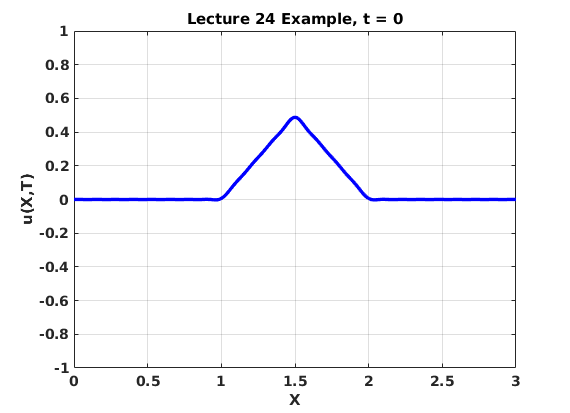
\includegraphics[width=2in]{lec24_t0.png}}
\subfloat[]{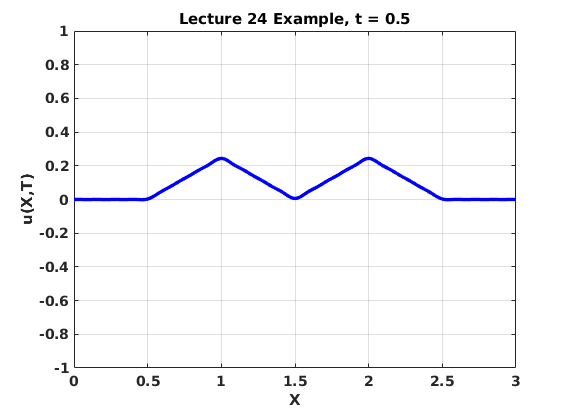
\includegraphics[width=2in]{lec24_t0p5.png}}
\subfloat[]{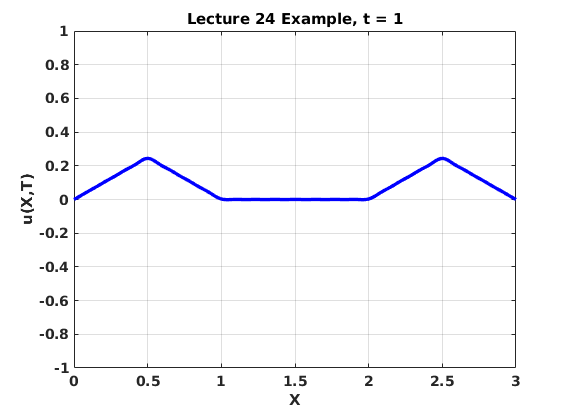
\includegraphics[width=2in]{lec24_t1p0.png}}
\\
\subfloat[]{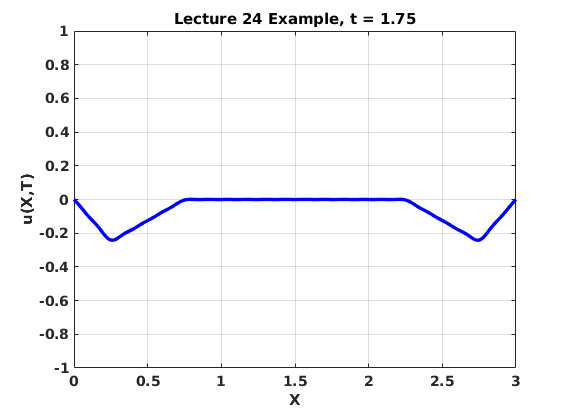
\includegraphics[width=2in]{lec24_t1p75.png}}
\subfloat[]{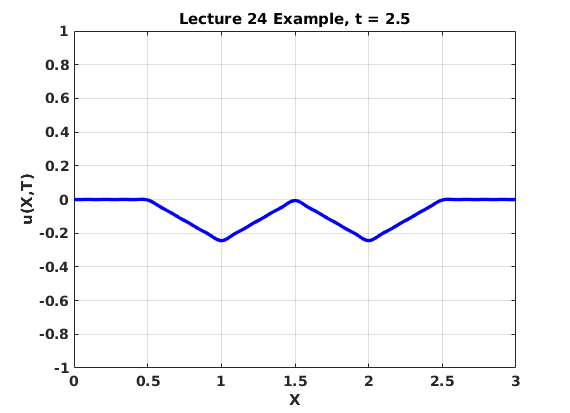
\includegraphics[width=2in]{lec24_t2p5.png}}
\subfloat[]{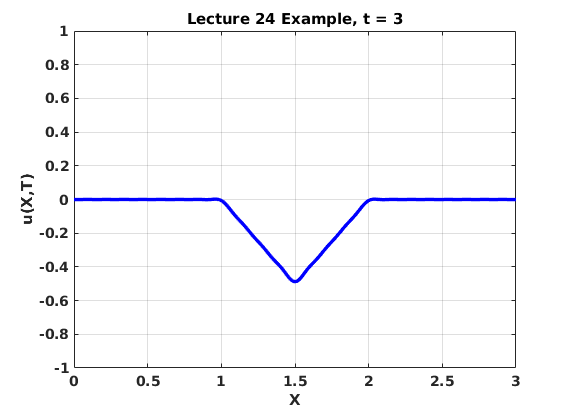
\includegraphics[width=2in]{lec24_t3p0.png}}
\label{fig:lec24-ex1}
\caption[][-1.0cm]{Wave equation solution from $t=0$ to $t=3$.}
\end{figure}
\end{fullwidth}

